\documentclass[BIT, graphvis, a4paper]{usydthesis}

\usepackage[final]{pdfpages} 
\usepackage[toc]{appendix}
\usepackage[utf8]{inputenc}
\usepackage{amsfonts}
\usepackage{amsmath}
\usepackage{amssymb}
\usepackage{caption} 
\usepackage{color} 
\usepackage{chngpage}
\usepackage{float}
\usepackage{framed}
\usepackage{fullpage}
\usepackage{titletoc}
\usepackage{graphicx}
\usepackage[a4paper,margin=1.3in,headheight=20pt,footskip=.6in,headsep=.2in]{geometry}
\usepackage{hyperref} 
\usepackage{listings} 
\usepackage{subcaption} 
\usepackage[
	backend=biber,
	natbib=true,
	style=numeric,
	url=true, 
	doi=true,
	eprint=false
]{biblatex}
\usepackage{tabularx} 
\usepackage{tabu} 
\usepackage{tikz} 
\usepackage{url}
\usepackage{wrapfig} 
\usepackage{fancyhdr}
\pagestyle{fancy}

\renewcommand{\sectionmark}[1]{\markright{\thesection.\ #1}}

\fancyhead{} % clear all header fields
\fancyhead[LO,LE]{\leftmark}
\fancyhead[RO,RE]{\thesection}

\fancyfoot{}
\fancyfoot[RO,LE]{\thepage}
\fancyfoot[LO,RE]{Linus Karsai}

\renewcommand{\headrulewidth}{0.4pt}

\addbibresource{bibliography.bib}

% Related work title/citation
\newcommand{\relatedwork}[1]{
	\textit{\citetitle{#1} \textcite{#1}}\\\\
	~
}


\usetikzlibrary{arrows}
\usetikzlibrary{shapes,snakes}
\usetikzlibrary{positioning,calc}
\DeclareUnicodeCharacter{00A0}{ }
\newcommand*\rot{\rotatebox{90}}
\makeatletter
\newcommand{\@chapapp}{\relax}%
\makeatother
\graphicspath{ {images/} }
\setlength{\parskip}{\baselineskip}%
\setlength{\parindent}{0pt}%
% graph settings
\definecolor{nodeyellow}{RGB}{255,252,135}
\definecolor{nodeblue}{RGB}{179,255,255}
\tikzset{
	every node/.style={font=\sffamily\scriptsize}
}
\tikzset{
	group/.style={font=\sffamily,fill=nodeblue}
}
\tikzset{
	->,>=stealth',shorten >=1pt,auto,node distance=3cm,
	thick,main node/.style={ellipse,fill=nodeyellow,draw,font=\sffamily\normalsize}
}

% give captions a bit of space.
\captionsetup[sub]{margin=5pt, skip=10pt}

% listings style for prov code
\lstdefinestyle{provn}{
	breaklines=true,
	showstringspaces=false,
	basicstyle=\footnotesize\ttfamily,
}
\lstdefinestyle{basic}{
	breaklines=true,
	showstringspaces=false,
	basicstyle=\footnotesize\ttfamily,
	keywordstyle=\color{black},
	commentstyle=\color{black},
	stringstyle=\color{black},
}


\title{Clustering Provenance}

\begin{document}
\author{Linus Karsai}

\pagenumbering{roman}
\maketitle
\chapter*{Contents}

\startcontents[sections]
\printcontents[sections]{l}{0}{\setcounter{tocdepth}{1}}

\chapter{Abstract}

As digital objects become increasingly important in people's lives, people may need to understand the 
\emph{provenance}, or lineage and history, of an important digital object,
to understand how  it was produced.
This is particularly important for objects created from large, multi-source collections of personal data.
As the metadata  describing provenance, Provenance Data, is commonly represented as a labelled directed acyclic graph,
the challenge is to create effective interfaces onto such graphs
so that people can understand the provenance of key digital objects.
This unsolved problem is especially challenging for the case of novice and intermittent users and
complex provenance graphs.

We tackle this by creating an interface based on a \emph{clustering} approach.
This was designed to enable users to view provenance graphs,
and to simplify complex graphs by combining several nodes.

Our core contribution is the design of an interface that supports clustering
and its analytic evaluation in terms of desirable properties of visualisation interfaces.
 % abstract of thesis

% reset the page numbering and change to arabic numbers
\newpage\setcounter{page}{1}\pagenumbering{arabic}

\chapter{Introduction}

Provenance as a concept has been around for a long time. It originally comes from the Latin word \textit{provenio}, meaning ``to come forth''. It's primary use is in the field of antiques where provenance is used to identify the authenticity and quality of something. For anyone with a backgruond in databases this term may also be fimilair as linking tuples in a query output to the reasons they exist.

In this paper the provenance we refer to is that of \textit{digital provenance}. It is a type of metadata representing the lineage of an object. Naively it can be compared to the information stored in revision history systems like that used in google docs\footnote{Google docs: \url{https://docs.google.com}} or version control
% TODO: git and mercurial links
systems such as git\footnote{GIT\: \url{}} or mercurial. These systems are usually limited to storing revisions as well as authorship. However extends beyond this by making it posible to store and ultimately trace what other things and activities led to a digital object been in its current state.

Provenance has the potential for usefulness in many different fields. The foremost and focus of this paper is the field of personal data management, allowing users to understand how their data is used. Often when a user chooses to share their personal data it is aggregated, anonymised or passed through any number of functions. By exploring provenance users have the ability to understand exactly how much and in what state their personal data is used.

An example to illistrate this point. Alice has a report that describes her current fitness level as well as outlining possible improvements. Viewing the provenance of
% TODO: Fitbit and Withings footnotes
this report shows which sources have been used (e.g. Fit-Bit data to track steps, Withings scale to track weight) and what processes analysed them. In this case it could show that Alice's fitness report was generated using step data from her FitBit data, passed through a summarisation process that summarises 15 minute interval data into daily steps. This shows tracing of lineage backwards in time, it is also possible to trace information forward, possibly in the case of errors in data. Alice remembers that she lent her FitBit to a friend to try for a week, causing errors in her data. Provenance would allow tracing of the errenous information forward to see what other processes and entities it effected and would need to be corrected.

Provenance is also potentially useful in any field where the lineage of an object needs to be stored. This could be extended to digital records of antiques or artwork. This would also be useful in data warehouse systems where information about data transformations as well as origin are stored. There is also research into storing provenance in
% TODO: reference to block chains
block-chains or similar systems to prevent medling of historical data where it to be used in high risk systems such as banks or accounting systems.

Early provenance systems stored provenance information in a variety of different flat
% TODO: prov reference
file formats. Since 2013, the PROV specification has provided a generic model for storing provenance with a number of serialisations (PROV-N, XML, JSON and RDF). PROV identifies provenance elements as three main concepts:

\begin{itemize}
	\item Entities: Physical, digital, conceptual objects
	\item Activities: Elements that cause an entity to come into existence
	\item Agents: Someone or something that can be assigned responsibility for an activity taking place.
\end{itemize}

The industry standard for representing these concepts is on an acyclic graph. An example of this with each of the three main concepts can be see in Figure~\ref{fig:key-concepts}.

\begin{wrapfigure}{r}{0.5\textwidth}
	\centering
	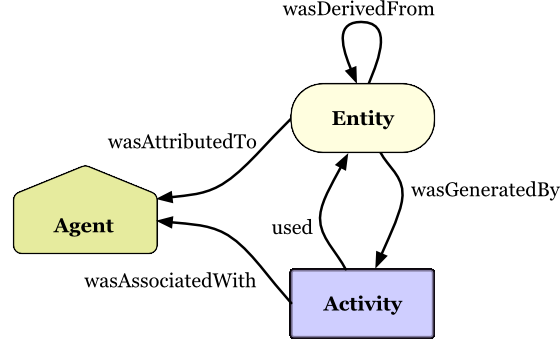
\includegraphics[width=\linewidth]{key-concepts}
	\caption{Key Concepts and relationships from the PROV standard displayed in a labelled acyclic graph.}
	\label{fig:key-concepts}
\end{wrapfigure}

Provenance can be stored in a variety of different granularity's and levels. The main three levels or provenance are system-level, application-level and network level. System level provenance is the lowest level and will often capture operating system activities such as which application ran at what to point to affect a piece of data. Application level provenance is limited to a single application, and will often capture information directly related to the user using that application. Network provenance captures information via network switches and stores lineage originating from multiple machines. These three levels are quire broad and do not cover all use cases but they do give a good point for starting discussion and comparing provenance capture tools. Provenance is also captured at different levels of granularity. Using the example of Alice as above, a system may capture information about her step data at the smallest granularity: how many steps every 15 minutes, or it may store the information at a larger granularity: aggregating step data daily.

As you can see in Figure~\ref{fig:key-concepts} provenance graphs are most often represented as directed acyclic graphs
% TODO: Novel provenance representation citing
although there has been some other novel approaches. The main problem we discuss is  provenance can become incredibly large, particularly in the case of OS level recording as it is usually at a low granularity so a lot of data is been recorded in a small time. Because provenance is inherently historical it is forever growing in size (as of yet there's no standard for going back and ``compressing'' history,) this means even  provenance captured as a high granularity will monotomiously grow and can become a graph with thousands or millions of nodes. This quickly becomes a
% TODO: usability studies chapter cite
usability problem as users can't visually digest such large graphs (results for usability studies in section x show that users are even put off by graphs with as little as 30 nodes).

What we describe in this paper is a process of simplifying graphs by clustering nodes into single composite nodes. A part from simplifying the graph and presenting less objects on screen, this also allows users to control what information is seen by other people or highlight particular concepts as seen in section x.
 % intro to pro etc.

\chapter{Clustering Interface Design}

% Clustering introduction, what is it, how does it work?
% Clustering nodes with mouse
% Cluserting with regex
% Useful naming of nodes
% Avoiding false dependencies

Clustering in this paper is the action of taking a set of nodes removing them from the graph and replacing them with a single composite node. An example of this is in Figure~\ref{fig:clustering-example} where you can see the node \textit{Fitness-Summary} and all its children have been clustered to create the composite node named `Fitness Data'. There is two primary ways of creating clusters, the first is automatically based on properties of the nodes or other heuristics, the second is via manual selection by the user. Previous research has been done into automatic clustering~\cite{Borkin2013,Seltzer2011}, what we focus on in this thesis is expanding on the work done in manual clustering~\cite{Biton2007} by designing an interface that allows effective clustering not just as a method of graph simplification, but as a way of conveying information.

The primary requirements for manual clustering where that it be simple to use and intuitive to new users. It should be easy for users to cluster nodes together without been shown how to. But it must also be powerful for expert users, so that someone who deals with provenance on a daily basis can quickly and easily create summary graphs with composite nodes in a minimal amount of time and effort.

\begin{figure}[h]
  \centering
  \begin{subfigure}[t]{0.5\textwidth}
    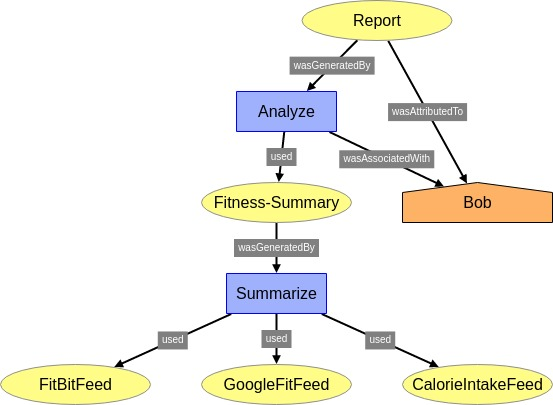
\includegraphics[width=0.9\textwidth]{clustering-example-2}
    \caption{The full provenance graph with no clustering.}
  \end{subfigure}
  ~
  \begin{subfigure}[t]{0.5\textwidth}
    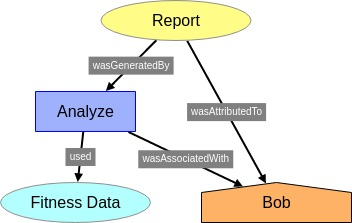
\includegraphics[width=0.9\textwidth]{clustering-example-1}
	\caption{The node \texttt{Fitness-Summary} and all its children have been grouped into a composite node \texttt{Fitness Data}}
  \end{subfigure}
  \caption{Above is a provenance graph showing the lineage of a report on Bob's fitness. On the left is the full graph, on the right a cluster has been manually created.}
  \label{fig:clustering-example}
\end{figure}

To fulfil these requirements I designed two different mechanisms for clustering, one for novice users and one for expert users. Although both can be used by either category of user it is easiest to differentiate them this way. 

\section{Manually clustering nodes}
\label{sec:user_defined_clusters}

The first method I designed was for novice users and works the following way: a user selects multiple nodes by clicking on them whilt holding down \textit{ctrl}, each selected node is outlined red as an indicater to the user that they are selected. Users can then cluster the nodes together by selecting a group function from a list of contextual actions. 

This allows users to cluster nodes together with little to no prompting from an expert. However it has the drawbacks of only been viable to a small number of nodes as selecting more than a dozen or so nodes is tedious and error prone. 

In order to allow precise and powerful node selection I designed a second way of allowing users to cluster nodes via a regex search function. Using the search bar users can input regex strings and matching nodes will be selected (same as manually clicking, selected nodes are outlined red). Once the user had tweaked the query to their liking they can group the nodes using the same technique as before; selecting the group function from a list of contextual actions. To make it easier to create multiple clusters quickly, pressing \textit{enter} while in the search field will cluster together the currently selected nodes, this allows users to quickly create a series of clusters without having to move their hands from the keyboard (a detailed analysis of the effectiveness of this can be found below in Section~\ref{sub:goms_analysis}). The regex query currently searches all properties and attributes of nodes, a future path of work would be to expand it so that you can match on specific properties.

Creating these two methods of clustering allows users to easily be introduced to the concept of clustering in an intuitive way, by clicking on nodes, then expand to the more complex and powerful tool of regex searching. Details on how these two methods where implemented can be found in Section~\ref{sec:clustering}.

\subsection{GOMS analysis}
\label{sub:goms_analysis}

GOMS is a method of assessing speed of use for expert users. In this case expert users are people who are trained in the field and used to using this application. It can be used to compare how long it takes to accomplish a tasks in different ways. In this case I use it to compare the speed difference between \textit{ctrl+click} clustering and search clustering.

A task is given a series of letters to represent what happens when a user tries to accomplish that task. For example, using the \textit{ctrl+click} method to select the nodes as shown in Figure~\ref{fig:clustering-example} would be: HMPCR HK MPCR MPCR MPCR MPCR MPCR. Each letter represents something that occurs:

\begin{itemize}
\item K - keypress
\item P - point with mouse
\item C - click with mouse
\item H - home hands on new device
\item M - mentally prepare
\item R(t) - system response time
\end{itemize}

So using this we can break down the GOMS string for \textit{ctrl+click} as meaning the follwing:

\begin{itemize}
	\item HMPCR - User moves hand to mouse and points and clicks at \texttt{Fitness-Summary} node (node is hilighted with red outline)
\item HK - User moves hand to keyboard and holds down \textit{ctrl} button
\item MPCR - User moves mouse and clicks the \textit{Summarise} node.
\item MPCR - User moves mouse and clicks the \textit{FitBitFeed} node.
\item MPCR - User moves mouse and clicks the \textit{GoogleFitFeed} node.
\item MPCR - User moves mouse and clicks the \textit{CalorieIntakeFeed} node.
\item RMKPCR - User sees group link in contextual actions, stops hodling down \textit{ctrl}, moves mouse to the group link and clicks it. The nodes move together and create a composite node.
\end{itemize}

Similarly, search clustering can be represented as the follwing: 

\begin{itemize}
\item HMC - User moves hand to mouse and selects the search button from the toolbar
\item RMPC - The search panel is show. The user moves the pointer and clicks the text input field of the search panel.
\item HMKKKKKKKKKKKKKK - User moves hands to the keyboard and types the following regex ``Summzarize|Feed''
\item KR - User presses \textit{enter}, the nodes move together and create a composite node.
\end{itemize}

We can then assign time values to each of these tasks as seen in Table~\ref{tab:goms-times} (this assumes that the system has instant response time). These times can then be used to calculate how long each tasks takes when conducted by an expert user.

\begin{table}[h]
	\centering
		\def\arraystretch{1.5}
	\caption{A list of GOMS tasks and their assosiated timing.}
	\label{tab:goms-times}
	\begin{tabular}{| c | l | c |}
		\hline
		\textbf{Letter} & \textbf{Desc.} & \textbf{Time (seconds)} \\
		\hline
		\hline
		K & keypress & .08 - 1.20 \\
		P & point with mouse & .8 - 1.5 (Fitt's Law) \\
		C & click with mouse & .2 \\
		H & home hands on new device & .4 \\
		M & mentally prepare & 1.35 \\
		R(t) & system response time & 0 \\
		\hline
	\end{tabular}
\end{table}

\begin{table}[h]
	\centering
		\def\arraystretch{1.5}
	\caption{The resulting times from GOMS analysis of the two methods for clustering a set of nodes, \textit{ctrl+clicking} and search clustering. I assume that it takes about 1.2 seconds for the user to point with the mouse, and that they're a moderately fast typer taking 0.2 seconds per keypress.}
	\label{tab:goms-results}
	\begin{tabular}{| l | l | c |}
		\hline
		\textbf{Method} & \textbf{GOMS string} & \textbf{Time (seconds)} \\
		\hline
		\hline
		Ctrl+click & HK MPCR MPCR MPCR MPCR RMKPCR & 14.54 \\
		Search group & HMC RMPC HMKKKKKKKKKKKKKK KR & 9.44 \\
		\hline
	\end{tabular}
\end{table}

As seen in Table~\ref{tab:goms-results} it takes approximately 15 seconds to conduct the grouping of \texttt{Fitness-Summary} and its children using the \textit{ctrl-click} method, while only taking 10 seconds when using the search group method. These results would vary depending on how fast a typer the user was and how good their fine motor skills where. It also depends on how ``searchable'' the nodes you wish to group are, in cases where the nodes have no common property values it may be faster to select the nodes using the \textit{ctrl-click} method. However in any case where the nodes you want to select share a property with the same value, the search group method is likely to come out on top because multiple nodes can be selected with a single string compared to having the limit of one node been selected by one click.

\section{Challenges}
\label{sec:naming_composite_nodes}

The main challenge in clustering nodes is that of naming. Once a composite node is created it must be given a name. In an early version of the ProvOwl system nodes where given short random alpha-numeric names. We found that this soon made the graph incomprehensible and relied on the user manually renaming each node (described in Section~\ref{sec:details_on_demand}) in order for the graph to be usable. 

Ideally an interface would give clusters a name describing its contents. I found this is a much harder problem than it at first seems and requires domain level knowledge as well as models of the user and what information is important to them. For example, the nodes \texttt{sunflower}, \texttt{daffodil} and \texttt{poppy} where to be clustered. Naively it would be useful to name the cluster \textit{plants}, however if the user was a florist this may be too broad a definition and the label \textit{flowers} would be more appropriate.

In some fields this problem has been solved by limiting the number of unknown things. For example, if you create a folder of apps on an iPhone it is automatically named with a label appropriate to the applications inside of it. A folder full of photography apps may be labelled \textit{Photography}. However this differs from the problem we are solving in a variety of ways. Firstly the number of possible labels is limited to the categories in the Apple app store, this creates a finite set of possible label options. Secondly, when an application is uploaded to the app store the author publishes metadata with it such as the category of the app. Using this metadata makes it much easier to name clustered items. Having the same level of metadata in provenance files could be accomplished by having tags associated with each node, these tags could then be used to effectively name a cluster simply by selecting the most used tag from the group of nodes to be clustered. However there is currently no tagging system for provenance nodes.

Our currently, still simple approach uses the name of the node in the cluster closest to the root with the text ``group'' appended to the end. While this doesn't always create the most effective names for clusters, it gives the user a point of reference when looking at clusters which in most cases is enough to trigger the user to what the contents of the cluster is. During usability studying users never renamed nodes unless they specifically wanted to convey information to another user.

\begin{figure}[h]
	\centering
	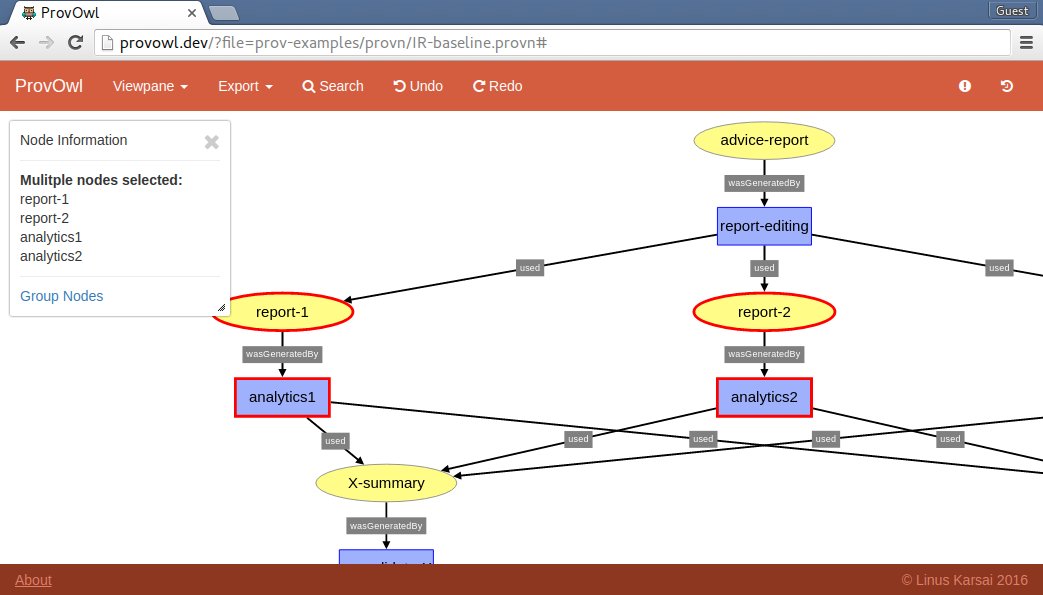
\includegraphics[width=\linewidth]{naming1}
	\caption{Using the \textit{IR-baseline} example the user has selected four nodes for grouping, essentially those related to \texttt{report-1} and \texttt{report-2}.}
	\label{fig:naming1}
\end{figure}
\begin{figure}[h]
	\centering
	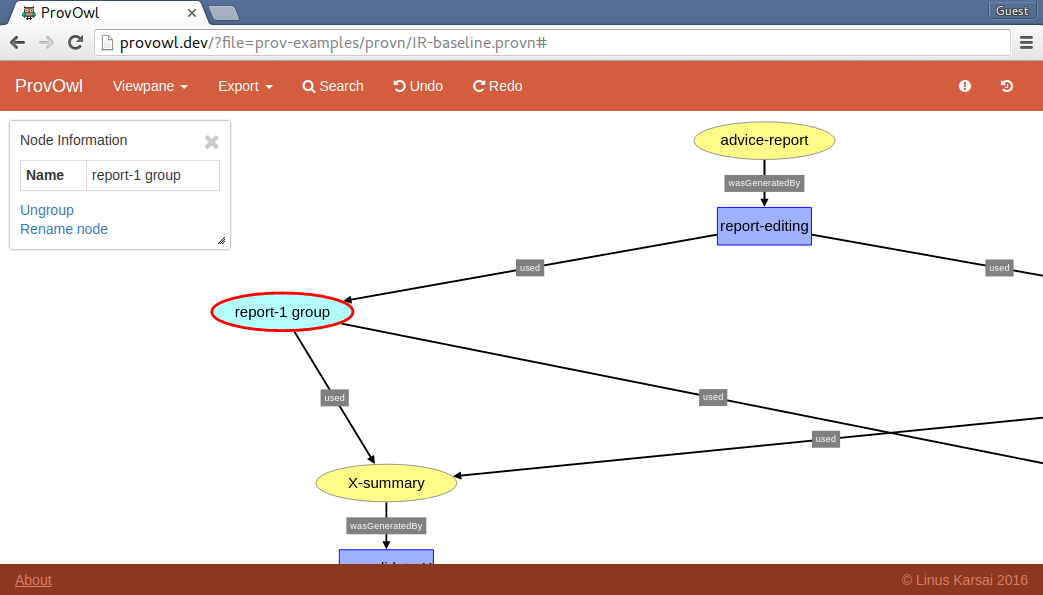
\includegraphics[width=\linewidth]{naming2}
	\caption{When clusterint the four nodes selected in Figure~\ref{fig:naming1} ProvOwl creates a composite node using the name of the node closest to the root (in this case breaking a tie by alphabetical order).}
	\label{fig:naming2}
\end{figure}
\clearpage

 % challenges of clustering

\chapter{Working Prototype}

In order to assess the effectiveness of the clustering techniques described above I decided to create a prototype application that would implement them. This prototype could then be used in usability studies to assess the effectiveness and usability of the clustering techniques. The prototype I created was a web application called ProvOwl, Figure~\ref{fig:interface-example} shows a screenshot of it open with one of the provenance files from the usability study. It reads provenance in the PROV-N format and renders a directed acyclic graph for users to interact with. ProvOwl is available to play with at \href{http://provowl.com/?file=prov-examples/provn/fitbit_score.provn}{ProvOwl.com} and the source code is available at \href{https://github.com/karsai5/ProvOwl}{github.com/karsai5/ProvOwl}. Below I go into detail about the features implemented in the prototype as well as information about the specifics of its implementation.

\begin{figure}[h]
\centering
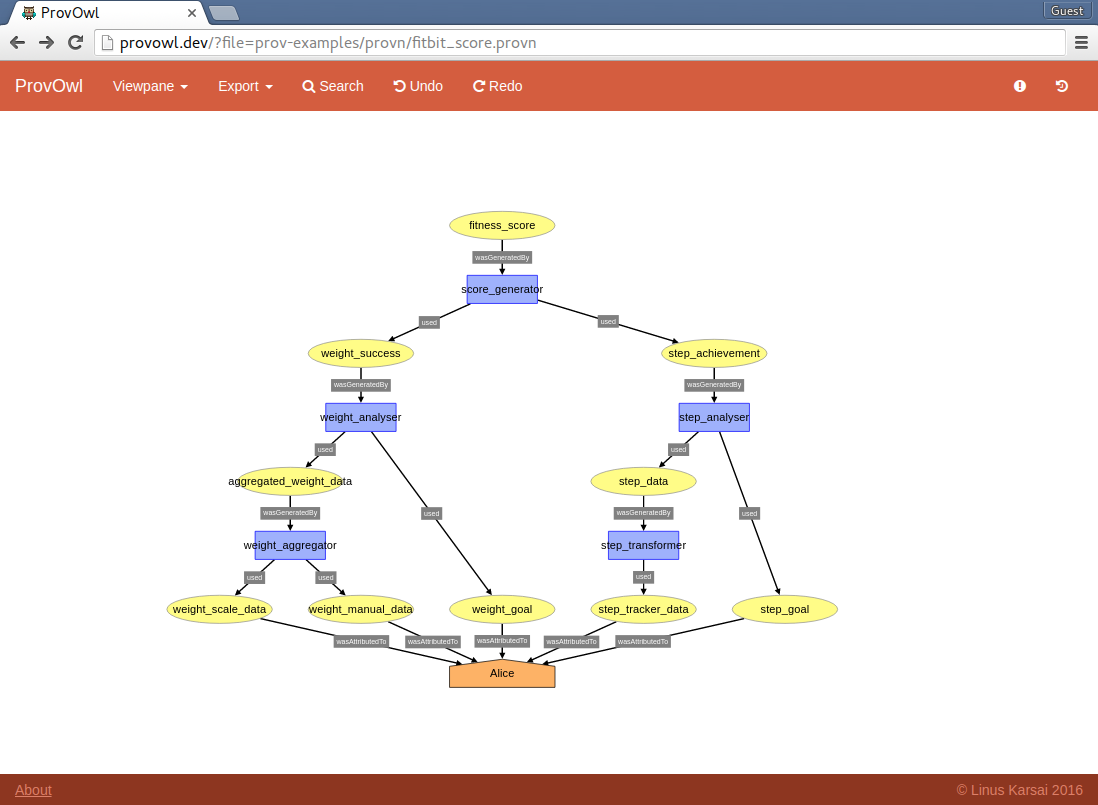
\includegraphics[width=\linewidth]{interface-example}
\caption{A screenshot of ProvOwl rendering the \texttt{fitbit\_score} prov file used in the usability studies.}
\label{fig:interface-example}
\end{figure}

\section{Functions and Design}

When creating the prototype I quickly discovered that the clustering functions could not be implemented in a vacuum and that a usable graph exploration tool would require other features as well. I used \citeauthor{Shneiderman1996}'s \citetitle{Shneiderman1996}~\cite{Shneiderman1996} as a starting point for creating a usable interface. In his paper he outlines seven usability tasks that should be taken into consideration when creating an advance graphical user interface. These where: \textit{Overview:} a user should be able to view the entire entity been visualised, this is important in giving them a sense of location and scale. \textit{Zoom:} When a user finds a point of interest they should be able to zoom in to view it in more detail. \textit{Filter:} Users should be able to limit what they see on screen to remove information they do not find useful. \textit{Deatils-on-demand:} A user should be able to view details about elements when they want. But the details should not be constantly on screen and cluttering the view. \textit{Relate:} Information between items should be visible; How information flows from one element to another. \textit{History:} Allow users to be able to undo and replay their actions, this is important in reassuring them that their actions are not permanent and they are free to make mistakes. \textit{Extract:} Once a user has found something interesting they should be able to extract their queries for later exploration or sharing.

Using these usability tasks as a starting point I implemented five main features. Each feature is described below as well as the reasoning behind implementing it and its relations to \citeauthor{Shneiderman1996}'s seven tasks.

\subsection{Movement and Rearranging}
\label{sec:movement_and_rearranging}

On first opening a provenance graph, the viewport is positioned to fit an entire graph on screen as seen in Figure~\ref{fig:interface-example}. This acomplishes the \textit{overview} task from above and allows the user to view all the provenance at once. Users can then pan around by clicking and dragging. Zooming is accomplished by pressing ctrl+[+,-] or by using the scroll wheel. In large graphs this allows users to zoom in on areas of interest. 

By default the graph's overall layout is detemined using a JavaScript library called dagre that generates layouts for directed acyclic graphs client side. The main skeleton of the algorithm implemented to acomplish this comes from the paper ``A technique for Drawing Directed Graphs''~\cite{Gansner1993}. In early prototypes other layout options where made available such as circle and breadth-first, but this confused users and where later removed in favor of using dagre exclusively for layout.

\begin{figure}[h]
	\centering
	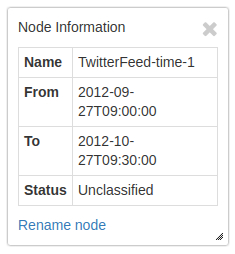
\includegraphics[width=5cm]{interface-details-close}
	\caption{A close up of the details panel from Figure~\ref{fig:interface-details}}
	\label{fig:key-concepts}
\end{figure}

Although initial placement is determined using the dagre algorithm, users can also re-arrange nodes manually by clicking and dragging a node. Note that this causes some issues when users are trying to pan, instead of cliking and dragging the background they accidentally click and move a node instead.

\subsection{Details on demand}
\label{sec:details_on_demand}

When a user selects a single or group of nodes the details panel is shown, as in Figure~\ref{fig:interface-details}. This displays information about the node as well as all its properties. At the bottom of the panel in blue text are contexual hyperlinks that enable functions such as renaming and in the case of multiple selected nodes, grouping. As suggested by the title, this directly immplements the taks of details-on-demand.

\begin{figure}[h]
	\centering
	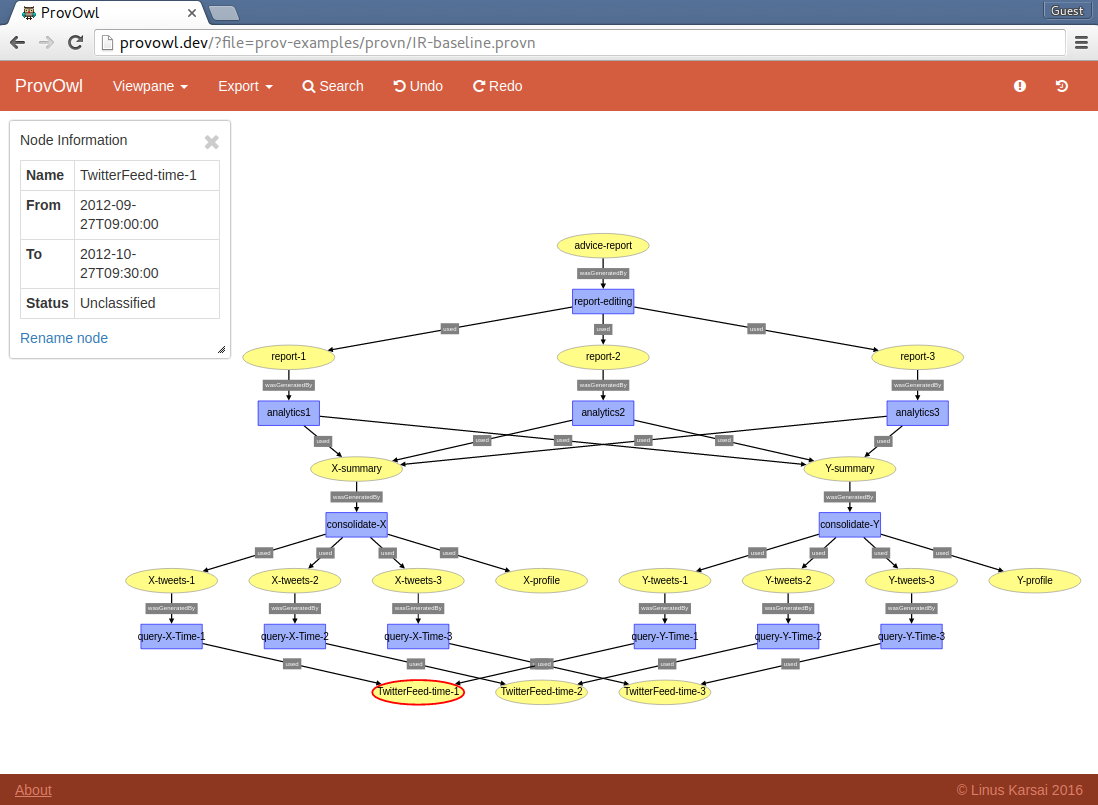
\includegraphics[width=\linewidth]{interface-details}
	\caption{A screenshot of ProvOwl with the \texttt{IR-baseline} prov file open. A indicated by the red outline, the node \texttt{TwitterFeed-time-1} has been selected and details about it such as name and classification status are shown in the details panel in the top left.}
	\label{fig:interface-details}
\end{figure}

\subsection{Clustering}
\label{sec:clustering}

As mentioned in Section~\ref{sec:user_defined_clusters} I have implemented two ways of clustering nodes, manually and via a search function. In both cases once the user activates the group function, the currently selected nodes are animated to their new position (the node closest to root) and replaced by a composite node, represented by a light blue oval. 

To manually cluster nodes a user first selects multiple nodes at once, by clicking on each whilst holding down \textit{ctrl}. Once multiple nodes have been selected the user cn group them together either with \textit{ctrl+g} or by selecting the group nodes hyperlink from the details panel.

The above method is tedious for more than a handful of nodes so I also implemented the search function. By opening up the search panel the user has access to a search field. The search function takes the value inputted by the user and runs a regex match on each property of each node. If any property of a node matches the regex it is selected (as indicated by a red outline).

In Figure~\ref{fig:search1} you can see an example of this. Open inside the ProvOwl interface is \textit{IR-baseline.prov}, an abstract example that shows the provenance of a report that is created to show analytical information about twitter data from two different users. On the right hand side of the screen is the search panel with the regex text \texttt{X-tweets|query-X-Time}. This query is run on all the nodes and because the pipe (\texttt{|}) characted represents an OR operator in regex hilights all the nodes that are either names \texttt{X-tweets-*} or \texttt{query-X-Time-*}. Once thses nodes are hilighted (as indicated by the red outline) they can be clustered into a composite node as seen in Figure~\ref{fig:search2}.


\begin{figure}[h]
	\centering
	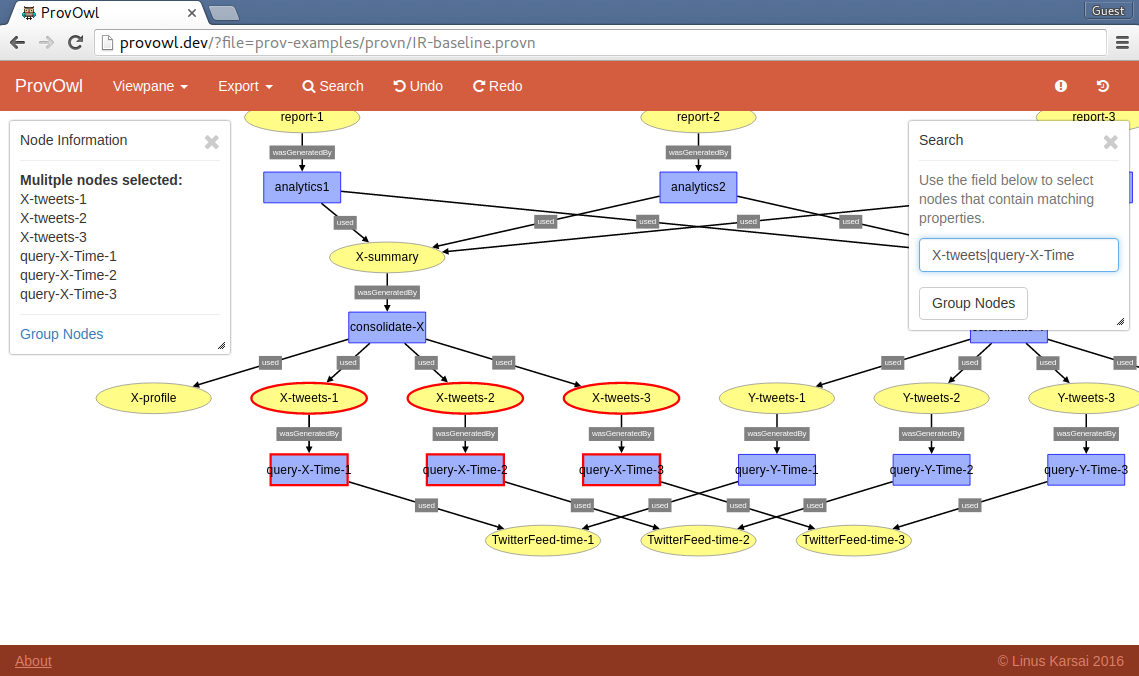
\includegraphics[width=\linewidth]{search1}
	\caption{A screenshot or ProvOwl with the \textit{IR-baseline.prov} file open; an abstract example that shows the provenance of an advice report presenting analytical information about twitter feeds. The search panel has been used to select a subset of the nodes.}
	\label{fig:search1}
\end{figure}
\begin{figure}[h]
	\centering
	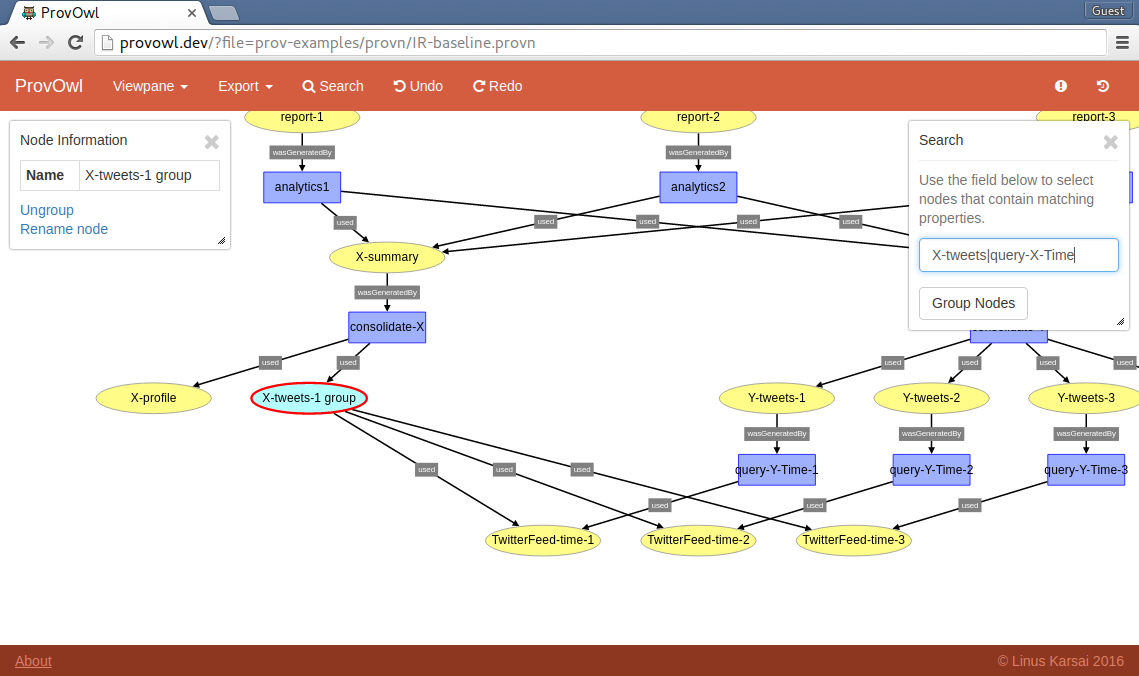
\includegraphics[width=\linewidth]{search2}
	\caption{Using the \textit{Group Nodes} button in the search panel, the nodes highlighted in Figure~\ref{fig:search1} have been clustered into a single composite node labelled \texttt{X-tweets-1 group}.}
	\label{fig:search2}
\end{figure}

\clearpage

\subsection{History}
\label{sec:history}

Having the ability to undo and redo actions is one of the above mentioned tasks for designing advance graphical interfaces and I believe one of the most important. It allows users to confidently and safely explore information without fear of causing permanent damage. My interface tracks primarily the movement and clustering of nodes. The undo and redo buttons allow users to step backwards and forwards through these actions. Using the history icon in the top right corner of the interface toggles a history pane (as seen in Figure~\ref{fig:interface-history}) that shows the user what step they are currently at. 

\begin{figure}[h]
	\centering
	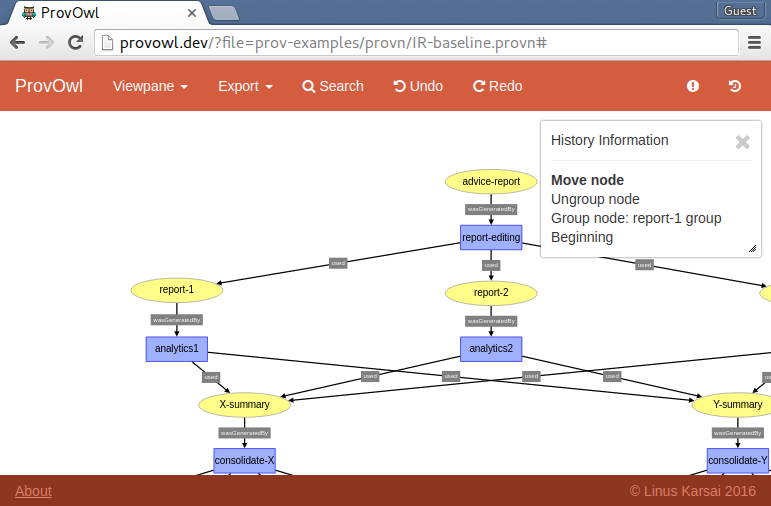
\includegraphics[width=0.8\linewidth]{interface-history}
	\caption{In the top right of the interface can be seen the history panel. This indicates what step of history the user is currently at. The user can use the undo and redo commands in the top bar to move backwards and forwards.}
	\label{fig:interface-history}
\end{figure}

\subsection{Sharing}
\label{sec:sharing}

In the top bar of Figure~\ref{fig:interface-history} there is a menu-bar option to export the current graph. This dropdown menu allows the user to either save the entire graph, or just the current viewport, as an image. The option to export just the viewport allows a user to focus on a certain section. This is related to the share task above and allows easy sharing of provenance files with other people for feedback and analysis. In the future I would also like to be able to export the current graph in PROV format with notation for clustered nodes.

\subsection{Click tracker}
\label{sec:click_tracker}

To facilitate with usability testing and by recommendation of Judy Kay I implemented a click tracker into the application. This simply logs clicks that the user makes, capturing time, location and element that the user clicked on. This could then be downloaded via the export command as a CSV file.  You can see below an example of the file generated from exploring the IR-baseline prov file.


\begin{figure}[h]
	\centering
	\lstinputlisting[style=basic]{misc/clickfile.csv}
	\caption{The CSV file generated from a user exploring the IR-baseline provenance file. Each line represent a single click by the user, a small description of the action they completed, what element it effected and the X,Y position of the click (if appropriate).}
	\label{fig:clickfile}
\end{figure}

\section{Implementation}

\subsection{Web Technologies}
\label{sec:web_technologies}

As we saw above, I implemented my prototype as a web application. The criteria for picking an implementation platform was that of accessibility to users and speed of development. Using that criteria I decided to make my prototype a web application as its only entry barrier to users is that of a modern web browser. I took the Prov-O-Vis~\cite{Hoekstra2014} system as inspiration as it was the most accesible of the availble provenance visualisers and this is partially because it is available online. Web applications are a field that I have experience with and can quickly develop in. 

There are a few pitfalls to this approach that can be addressed through alternative implementations. Because my application is primarily a prototype for illustrating effective exploration features, the issue of scale is not one that is addressed. If a web application was used for enterprise size provenance files the application may run out of resources; further testing and alternative approaches may be required.

An alternative to a web application would be to write the prototye in an OS independent language such as Java or Python; this would allow wide accessibility and more fine grained control of machine resources. However if an OS level language was chosen issues could later occur in presenting provenance on mobile devices and a mobile version of the interface may need to be written. Alternatively if an OS dependant language such as Apple's swift of Microsoft's C\# was used features and code would have to be replicated for the different OS languages (assuming that OS independent accessibility is an important criteria).

The standard technology for data visualisation in a browser is the D3.js\footnote{D3: Data Driven Documents \url{https://d3js.org/}} JavaScript library. However as mentioned earlier, I used Cytoscape.js to implement my interface because it is specifically focused on graph theory and has a graph functions built in (such as distance algorithms). 

\subsection{Client Side Processing}
\label{sec:client_side_processing}

When a provenance file is selected ProvOwl loads the file and renders it all locally. When first outlining features of the application I wanted it to be primarily stand alone. This means that even though it can run from a web server, you could just as easily run it locally on your computer with minimal effort as all computations are done client side.

However server side computation may be a useful feature for the future, a server with higher computational power and resources may be able to find and analyze interesting details about a file. A simple approach to accomplish this would to have the file uploaded to the server, analytics run on the provenance and then results loaded back to the client. For larger provenance files this could be extended to only load sections required for analysis reducing the bandwidth required. The client could render the provenance locally whilst results where computed and then rendered onto the already drawn graph. This would allow the user to begin exploring the graph with minimal delay while extra information is calculated server side.

\subsection{Node Clustering}

Creating a clustering functino in Cytoscape.js required some time and effort because it currently doesn't have a clustering feature, so I was required to write one from scratch. The goal of this function was to have grouping and ungrouping nodes been undestructive: if a series of nodes are grouped and then ungrouped the resulting graph should be isomorphic to the original.

\begin{figure}[h]
  \centering
  \begin{subfigure}[t]{0.5\textwidth}
    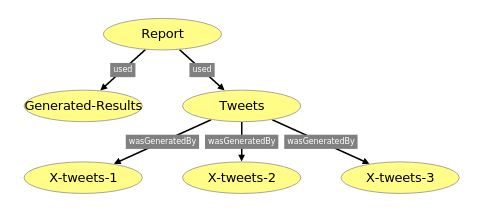
\includegraphics[width=\textwidth]{ungrouped}
    \caption{A provenance graph showing information about a report given on twitter data.}
  \end{subfigure}
  ~
  \begin{subfigure}[t]{0.5\textwidth}
    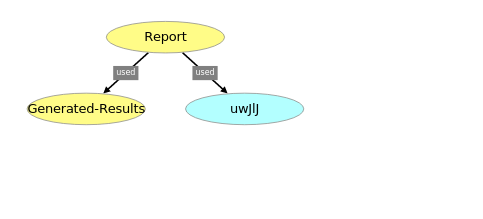
\includegraphics[width=\textwidth]{grouped}
	\caption{The nodes \texttt{Tweets} and \texttt{X-tweets-[1-3]} have been clustered into the composite node \texttt{uwJIJ}}
  \end{subfigure}
  \caption{A provenance that has had a subset of its nodes clustered. In an early version of the prototype composite nodes were given random alphanumeric names as seen on the right.}
\end{figure}

Nodes removed from Cytoscape.js can be `restored' into their original position, unfortunately any edged associated with a removed node are permanently destroyed. It is necessary then to store the edges as a data field in the composite node so that when restoring nodes, edges can also be recreated. 

The pseudocode below creates a new cluster. It creates a new node and stores the selected nodes and their edges as properties of it. Then new edges are created from surrounding nodes to the composite node. Finally the selected nodes are ``removed'' so that they are no longer visible.

\begin{figure}[h]
  \centering
  \begin{lstlisting}
 // Create composite node 
 Create new CompositeNode 
 CompositeNode.originalEdges = All edges in neighbourhood of selected nodes // save edges
 CompositeNode.originalNodes = All nodes that where grouped // save nodes

 // Create new edges connected to the composite node
 for each edge in neighbourhood {
  if (edge IS NOT internal to group)  {
    Create new Edge({from: externalNode, to:compositeNode})
  }
 }

 // Remove original nodes
 Remove selected nodes
 \end{lstlisting}
 \caption{Pseudocode: Creaing a composite node}
\end{figure}

However the above code only works in a limited scenario: ungrouping nodes in the opposite order of creation. For example if you created composite nodes $A$, $B$, $C$ (chronologically and all with neighbouring edges) you would have to ungroup them in the following order: $C$, $B$, $A$. If you where to for example ungroup node $A$ first, when ungrouping $C$ it would try to restore edges to the now non-existenat $A$ compsosite node, there's an example of this in Figure~\ref{fig:clustring-without-groupmanager}. In order to fix this I created a class called group manager to monitor nodes in clusters.

The Group Manager class is the primary way of keeping track of nodes that are hidden inside composite nodes. It contains a tree data structure that references all the groups as well as their child nodes/groups. When ungrouping nodes this class is called and the parent group of the child node requested, then a new temporary edge is created to the composite node and the original edge stored in a \textit{hanging edges} object until it can be restored. Every time a group is created or destroyed the \textit{hanging edges} object is queried to see if any originl edges can be recreated, as seen in Figure~\ref{fig:clustring-with-groupmanager}.

\begin{figure}[h]

  \begin{subfigure}[t]{0.5\textwidth}
    \centering
    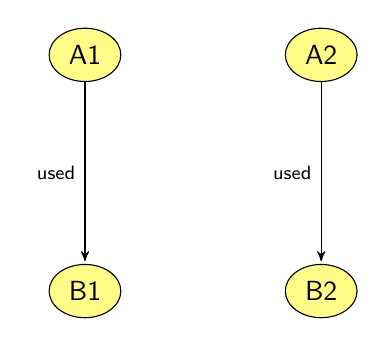
\begin{tikzpicture}
      \node[main node] (A1) {A1};
      \node[main node] (A2) [right of=A1] {A2};
      \node[main node] (B1) [below of=A1] {B1};
      \node[main node] (B2) [below of=A2] {B2};
      \path (A1) edge node[left] {used} (B1);
      \path (A2) edge node[left] {used} (B2);
    \end{tikzpicture}
    \caption{Nodes $A1$ and $B1$ are linked, nodes $A2$ and $B2$ are linked.}
  \end{subfigure}
  ~
  \begin{subfigure}[t]{0.5\textwidth}
    \centering
    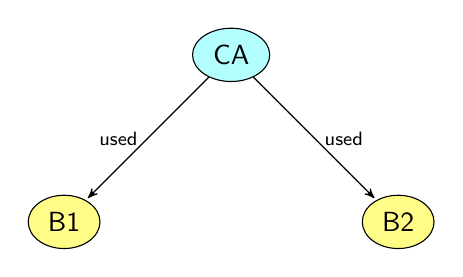
\begin{tikzpicture}
      \node[main node, group] (CA) {CA};
      \node[main node] (B1) [below left of=CA] {B1};
      \node[main node] (B2) [below right of=CA] {B2};
      \path (CA) edge node[left] {used} (B1);
      \path (CA) edge node[right] {used} (B2);
    \end{tikzpicture}
    \caption{Group nodes $A1$ and $A2$ into composite node $CA$. Stored inside the composite node is the original edges from $A1\rightarrow B1$ and $A2\rightarrow B2$.}
  \end{subfigure}
  \begin{subfigure}[t]{0.5\textwidth}
    \centering
    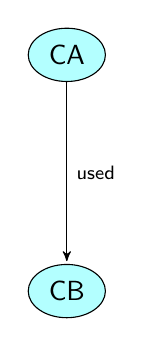
\begin{tikzpicture}
      \node[main node, group] (CA) {CA};
      \node[main node, group] (CB) [below of=CA] {CB};
      \path (CA) edge node[right] {used} (CB);
    \end{tikzpicture}
    \caption{Group nodes $B1$ and $B2$ insto composite nodes $CB$. Stored inside the composite node $CB$ is the edges from $CA\rightarrow B1$ and $CA\rightarrow B2$.}
  \end{subfigure}
  ~
  \begin{subfigure}[t]{0.5\textwidth}
    \centering
    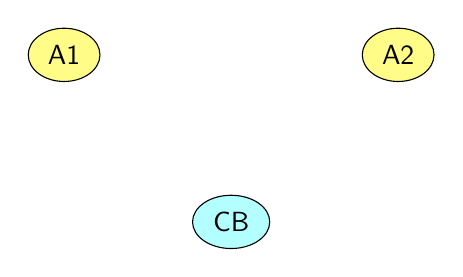
\begin{tikzpicture}
      \node[main node, group] (CB) {CB};
      \node[main node] (A1) [above left of=CB] {A1};
      \node[main node] (A2) [above right of=CB] {A2};
    \end{tikzpicture}
    \caption{Ungroup $CA$. It will try to create adges between $A1\rightarrow B1$ and $A2\rightarrow B2$, because $B1$ and $B2$ are currently in a group, the new edges will fail and not be rendered.}
  \end{subfigure}
  \begin{subfigure}[t]{0.5\textwidth}
    \centering
    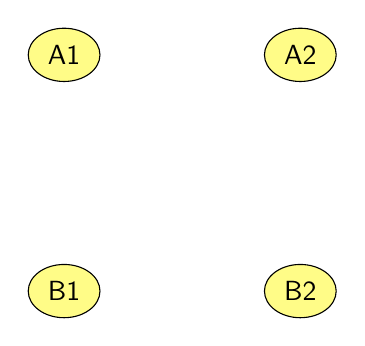
\begin{tikzpicture}
      \node[main node] (A1) {A1};
      \node[main node] (A2) [right of=A1] {A2};
      \node[main node] (B1) [below of=A1] {B1};
      \node[main node] (B2) [below of=A2] {B2};
    \end{tikzpicture}
    \caption{Ungroup $CB$. Edges between $CA\rightarrow B1$ and $CA\rightarrow B2$ will try to be restored but because there's no $CA$ in the graph these will fail.}
  \end{subfigure}
  \caption{An example of issues that occur when trying to ungroup nodes in the incorrect order without the \textit{Group Manager}. As seen in the final step, the original edges connecting the nodes are lost.}
\end{figure}

% ------------------
% BEGIN GIANT FIGURE
% ------------------

\newgeometry{top=2cm}
\begin{figure}[h]

  \begin{subfigure}[t]{0.5\textwidth}
    \centering
    \renewcommand\thesubfigure{A1}
    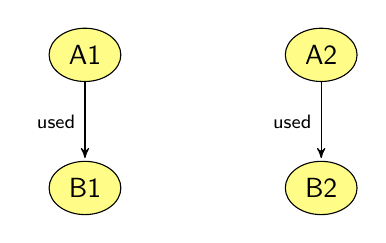
\begin{tikzpicture}
      \node[main node] (A1) {A1};
      \node[main node] (A2) [right of=A1] {A2};
      \node[main node] (B1) [below = 1cm of A1] {B1};
      \node[main node] (B2) [below = 1cm of A2] {B2};
      \path (A1) edge node[left] {used} (B1);
      \path (A2) edge node[left] {used} (B2);
    \end{tikzpicture}
    \caption{Nodes $A1$ and $B1$ are linked, nodes $A2$ and $B2$ are linked.}
  \end{subfigure}
  ~
  \begin{subfigure}[t]{0.5\textwidth}
    \renewcommand\thesubfigure{A2}
    \centering
    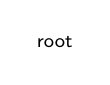
\begin{tikzpicture}
      \node[] (root) {root};
    \end{tikzpicture}
    \caption{The GMTree (Group Manager Tree) is currently empty and Hangingedges = [].}
  \end{subfigure}
  \begin{subfigure}[t]{0.5\textwidth}
    \centering
    \renewcommand\thesubfigure{B1}
    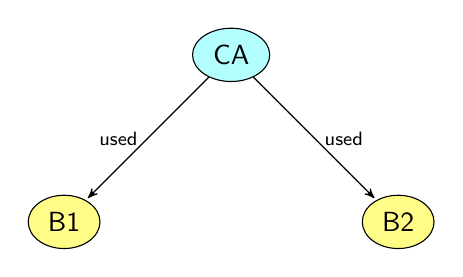
\begin{tikzpicture}
      \node[main node, group] (CA) {CA};
      \node[main node] (B1) [below left of=CA] {B1};
      \node[main node] (B2) [below right of=CA] {B2};
      \path (CA) edge node[left] {used} (B1);
      \path (CA) edge node[right] {used} (B2);
    \end{tikzpicture}
    \caption{Group nodes $A1$ and $A2$ into composite node $CA$. Stored inside the composite node is the original edges from $A1\rightarrow B1$ and $A2\rightarrow B2$.}
  \end{subfigure}
  ~
  \begin{subfigure}[t]{0.5\textwidth}
    \centering
    \renewcommand\thesubfigure{B2}
    \begin{tikzpicture}
      \node[] (root) {root};
      \node[below = 1cm of root] (CA) {CA};
      \node[below right = 1cm of CA] (A1) {A1};
      \node[below left = 1cm of CA] (A2) {A2};
      \path (root) edge (CA);
      \path (CA) edge (A1);
      \path (CA) edge (A2);
    \end{tikzpicture}
    \caption{The GMTree holds information about $CA$, $A1$ and $A2$. Hangingedges = [].}
  \end{subfigure}

  \begin{subfigure}[t]{0.5\textwidth}
    \renewcommand\thesubfigure{C1}
    \centering
    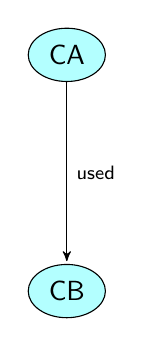
\begin{tikzpicture}
      \node[main node, group] (CA) {CA};
      \node[main node, group] (CB) [below of=CA] {CB};
      \path (CA) edge node[right] {used} (CB);
    \end{tikzpicture}
    \caption{Group nodes $B1$ and $B2$ insto composite nodes $CB$. Stored inside the composite node $CB$ is the edges from $CA\rightarrow B1$ and $CA\rightarrow B2$.}
  \end{subfigure}
  ~
  \begin{subfigure}[t]{0.5\textwidth}
    \centering
    \renewcommand\thesubfigure{C2}
    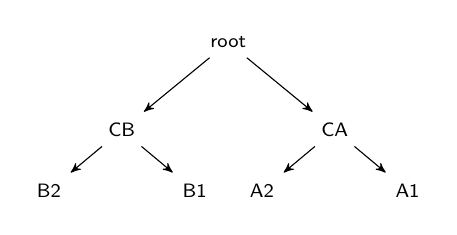
\begin{tikzpicture}
      \node[] (root) {root};
      \node[below right = 1cm of root] (CA) {CA};
      \node[below right = 0.5cm of CA] (A1) {A1};
      \node[below left = 0.5cm of CA] (A2) {A2};

      \node[below left = 1cm of root] (CB) {CB};
      \node[below right = 0.5cm of CB] (B1) {B1};
      \node[below left = 0.5cm of CB] (B2) {B2};
      \path (root) edge (CA);
      \path (CA) edge (A1);
      \path (CA) edge (A2);
      \path (root) edge (CB);
      \path (CB) edge (B1);
      \path (CB) edge (B2);
    \end{tikzpicture}
    \caption{The GMTree holds information about all nodes. Hangingedges = [].}
  \end{subfigure}

  \begin{subfigure}[t]{0.5\textwidth}
    \centering
    \renewcommand\thesubfigure{D1}
    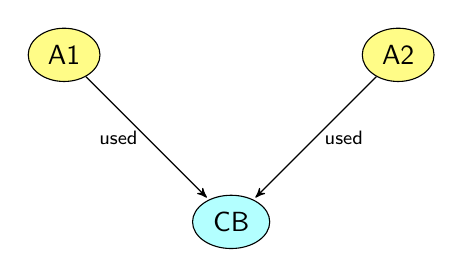
\begin{tikzpicture}
      \node[main node, group] (CB) {CB};
      \node[main node] (A1) [above left of=CB] {A1};
      \node[main node] (A2) [above right of=CB] {A2};
      \path (A1) edge node[left] {used} (CB);
      \path (A2) edge node[right] {used} (CB);
    \end{tikzpicture}
    \caption{CA is ungrouped and removed from the group manager tree. The original edges $A1\rightarrow B1$ and $A2\rightarrow B2$ can not be restored because B1 and B2 aren not in the graph, these edges are stored in the hanging edges object. New edges are created by finding the prent node using the group manager.}
	\label{fig:clustring-without-groupmanager}
  \end{subfigure}
  ~
  \begin{subfigure}[t]{0.5\textwidth}
    \centering
    \renewcommand\thesubfigure{D2}
    \begin{tikzpicture}
      \node[] (root) {root};
      \node[below = 1cm of root] (CB) {CB};
      \node[below right = 0.5cm of CB] (B1) {B1};
      \node[below left = 0.5cm of CB] (B2) {B2};
      \path (root) edge (CB);
      \path (CB) edge (B1);
      \path (CB) edge (B2);
    \end{tikzpicture}
    \caption{The GMTree holds information about $B$ nodes. $A$ nodes have been remove because they've been ungrouped. Hangingedges = [$A1\rightarrow B1$, $A2\rightarrow B2$].}
  \end{subfigure}

  \begin{subfigure}[t]{0.5\textwidth}
    \centering
    \renewcommand\thesubfigure{E1}
    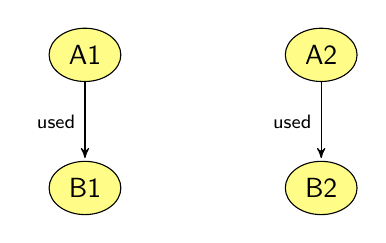
\begin{tikzpicture}
      \node[main node] (A1) {A1};
      \node[main node] (A2) [right of = A1] {A2};
      \node[main node] (B1) [below = 1cm of A1] {B1};
      \node[main node] (B2) [below = 1cm of A2] {B2};
      \path (A1) edge node[left] {used} (B1);
      \path (A2) edge node[left] {used} (B2);
    \end{tikzpicture}
    \caption{CB is ungrouped and removed from the group manager tree. An attempt to restore hanging edges is made and both $A1\rightarrow B1$ and $A2\rightarrow B2$ are restored.}
  \end{subfigure}
  ~
  \begin{subfigure}[t]{0.5\textwidth}
    \centering
    \renewcommand\thesubfigure{E2}
    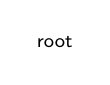
\begin{tikzpicture}
      \node[] (root) {root};
    \end{tikzpicture}
    \caption{The GMTree is empty because there's no groups. Hangingedges = [] because the previously stored edges have been restored.}
  \end{subfigure}
  \caption{The same example as in Figure~\ref{fig:clustring-without-groupmanager} except this time using the group manager and hanging edges. The group manager stores a tree to track groups and internal nodes as seen on the right hand side. Hanging edges stores a list of edges that have not been restored yet because one or more connected nodes were missing.}
	\label{fig:clustring-with-groupmanager}
\end{figure}

\restoregeometry % put geometry back to normal
 % technical implementation decisions

\chapter{Usability study}

In this paper I have so far described my first contribution: a design for manually clustering nodes and my second contribution a working prototype that implements those designs. My final contribution in the field of provenance is a usability study to evaluate learnability, ease of use, efficiency, recovery from errors and user attitude towards my prototype. I particularly felt that this was a requirement for designing an interface because unless an interface is usable it can not be useful. Below I go into details about the design of the study then in the next section I discuss the results.

\section{Study Design}
\label{sec:study_design}

\label{sec:interview_format}

I decided to conduct a think aloud study with participants while using the ProvOwl application. A think aloud involves having a user try to accomplish a set of tasks whilst you watch and take notes. Jakob Nielsen, a researcher specialising in discount usability engineering, describes it as the following:

\begin{quote}
``In a thinking aloud test, you ask test participants to use the system while continuously thinking out loud — that is, simply verbalizing their thoughts as they move through the user interface.'' 
\end{quote}

Participants are encouraged to ``think aloud'' as they complete tasks to give incite into what they are thinking. I selected this approach for a number of reasons. Firstly, it has been used successfully for a long time. \citeauthor{nielsen1994} describes it as ``...the single most valuable usability engineering method.'' in his 1993 book \citetitle{nielsen1994}~\cite{nielsen1994}. Secondly, it requires a small number of users to get meaningful results. A post written in 2012 by \citeauthor{nielsen1994} describes why you only need to test with five users\footnote{Thinking Aloud: The #1 Usability Tool: \url{https://www.nngroup.com/articles/thinking-aloud-the-1-usability-tool/}}. And lastly, I have conducted think aloud studies previously, so they are a natural first thought to me when gauging how usable an interface is.

Below I discuss the general format of the interviews and then in detail each of the scenarios users undertook and the tasks associated with each. The entire questionnaire I used for conducting the interviews can be seen at \ref{sec:interview_questionnaire}.


\subsection{Interview format}

The interviews were undertaken wherever was most convenient to the participant, this included at my desk, at the participants house or at coffee shops. The participants were asked a series of background questions, then undertook three scenarios in a think aloud study and finally were asked to complete a system usability scale questionnaire.

\subsubsection{Background Information}
\label{sec:background_information}

General background information was collected about each participant. Gender, age group and highest level of education. These were recorded in order to identify any demographic skew that I may have in my cohort as well as in case any unexpected correlations occurred. The last question in this background survey asked if the participant had heard of the term \textit{provenance} before, and if so to explain what it meant. Because provenance is used in other fields (such as accounting and art dealership) I wanted to identify anyone who had previous concepts of provenance and lineage to identify if this effected their ability to interpret provenance graphs.

\subsubsection{scenarios}

After the participant had answered the general background questions they were given a information sheet that explained the concept of provenance and showed an example of a provenance graph, explaining what each of the different coloured and shaped nodes meant (\ref{sec:prov_primer}). This allowed participants to have a uniform understanding of the concept of provenance regardless of whether they had heard of it before. Notes were taken of any questions the participant had whilst reading the information sheet.

They were then given my laptop. If the participant was not used to using a touchpad they were also supplied with a USB mouse. Open in a full screen browser was three tabs, one for each scenario the participant had to complete. Each scenario then has a series of tasks they had to either answer or complete, in some cases users required prompting to complete a task, in these cases I noted that the task was completed but with help. Each of the scenarios and tasks are discussed in detail in Section~\ref{sec:scenarios}.

\subsubsection{SUS Questionnaire}
\label{sec:sus_questionnaire}

The System Usability Scale has been around since 1996 when it was described by \citeauthor{brooke1996} in the paper \citetitle{brooke1996}~\cite{brooke1996} and provides a quick easy way of identifying if an interface is easy to use or not. It consists of 10 questions each requiring a response on a scale of 1--5. Users are asked to reply with what they intuitively feel rather than thinking about the questions for an extended period. 

I decided to use the SUS questionnaire because it is easy to administer (takes less than five minutes for users to complete), is valid in differentiating between usable and unusable interfaces~\cite{sauro2011} and can be used on a small sample size with reliable results\footnote{The usability.gov website has a good description of what a SUS questionnaire is and how to use it: https://www.usability.gov/how-to-and-tools/methods/system-usability-scale.html}.

\subsubsection{Coded questions}
\label{sec:coded_questions}

Each question was given a set of points, user actions that could be checked off if a user did them. For example, in question one of exercise one, the participant was asked \textit{What infroation is used to calculate your [fitness] score?}. One of the points for this question was \textit{ungrouped nodes}, so if the user ungrouped nodes while answering the question this point was ticked off. Whilst hand written notes were also taken during interviews, these checkboxes made for an easy way of identitying what common actions users undertook to complete exercises. 

Each point was assigned a code identifying what class of activity it belonged to. In the above example the ungrouping point had the code \textit{grouping-ungroup} because it's completing a grouping function and in particular an ungrouping function. 

Each of the codes are listed in Table~\ref{tab:question-codes} (page~\pageref{tab:question-codes}) with an explanation of the user behaviour they map to.

\subsection{Scenarios}
\label{sec:scenarios}

The user was asked to undertake three different scenarios, each with its own provenance file and a set of related tasks. Using multiple scenarios allowed me to have tasks that focussed on different objectives, for example the first scenario focuses on provenance understanding whilst the second and third are on provenance modification.

\subsubsection{Scenario 1: Alice's Fitness Score}
\label{ssub:scenario_1_alice_s_fitness_score}

In the first scenario the user is asked to imagine that they're Alice, they track their fitness information with a Fitbit for steps and a Withings scale for weight (images were shown to describe these objects as seen in \ref{sec:information_sheet}). The full paragraph given to participants:

\begin{framed}
Suppose you are Alice. You have been using your FitBit and Withings scales for 3 years to reduce your weight to 61kg and to increase your physical activity to 8000 steps a day. You have just linked your FitBit account to two friends, Bob and Carol. Recently FitBit introduced a fitness score that is shared and ranked with your friends\textellipsis This makes you wonder just how your score has been calculated.
\end{framed}

They were then asked to complete the following tasks, all of which required only a verbal answer.
\begin{enumerate}
	\item What data about you is used to calculate your score?
	\item Identify what aspects of the provenance graph map to your fitness dashboard.
	\item What processes does your raw step data go through before been used to calculate the fitbit\_score?
	\item How do you expect your raw fitbit data would be represented once it got to score\_generator?
	\item What processes does your Withings scale data go through before been used to calculate the fitbit\_score?
	\item How do you expect your weight data would be represented once it got to score\_generator?
	\item Are you concerned about how you data is used to calculate the fitbit score. Explain your reasoning. 
\end{enumerate}

The provenance graph they were given to answer these tasks can be seen in Figure~\ref{fig:exercise1a}. It can be seen from the light blue circles that this included composite nodes. I did this so that users were required to uncluster nodes (either by double clicking or selecting ``ungroup'' from the contexual commands) in order to properly answer the tasks. This meant that users were introduced to the idea of clustering before having to create them themselves in later tasks. These tasks also allowed the user to get used to reading provenance graphs. Questions C,D and E,F mirror each other so that if the user had difficulty understanding the way lineage worked in tasks C,D, requiring prompting. They could then accomplish D,E on their own. The last question G was simply a way of gauging what users found important, whether they where concerned about privacy or transparency in calculations.

This scenario was purely exploration based and no modifications of the graph where required in order to complete the tasks.

\begin{figure}[h]
	\begin{subfigure}[t]{0.4\textwidth}
	\centering
	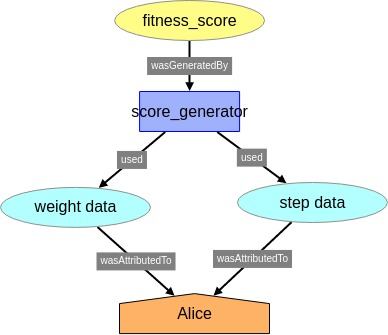
\includegraphics[width=\linewidth]{exercise1a}
	\caption{Alice's fitness score provenance with clusters.}
	\label{fig:exercise1a}
	\end{subfigure}
	\begin{subfigure}[t]{0.4\textwidth}
	\centering
	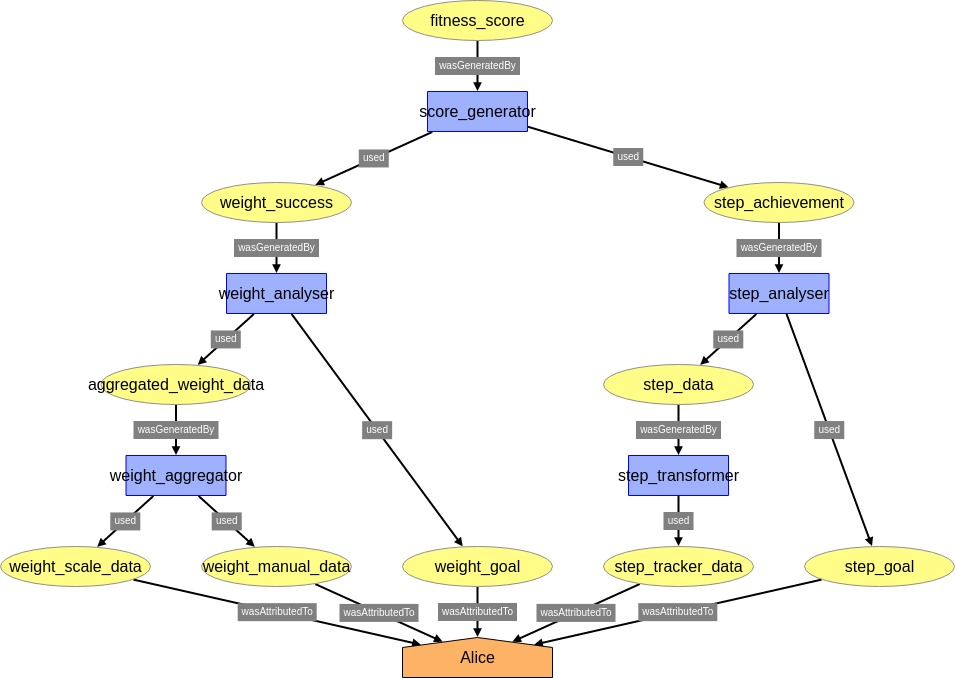
\includegraphics[width=\linewidth]{exercise1b}
	\caption{Alice's fitness score provenance without clusters.}
	\end{subfigure}
	\caption{The provenance graph used in scenario one showing the lineage of Alice's fitness score. The graph began with clusters as seen on the left. Completely unclustered the graph resembled that on the right.}
\end{figure}

\subsubsection{Scenario 2: Citizen Data Report}
\label{ssub:Scenario 2: Citizen Data Report}

The second exercise involved a larger amount of data and asked participants to imagine themselves as the curator of a citizen science project. Data was been tracked about multiple users and then used in a report that gave feedback on how to improve the cohorts overall fitness. The full paragraph given to participants:

\begin{absolutelynopagebreak}
\begin{framed}
You are a researcher creating a citizen-data-report that recommends strategies for improving the fitness of your local community. You have step, location, weight and calorie information about members of the community. You are using this information to create multiple reports regarding fitness and weight information which will be used to support a final report addressed to the community on strategies that can be used to improve overall fitness. 
\end{framed}
\end{absolutelynopagebreak}

They were then asked to compete the following tasks. 

\begin{enumerate}
	\item Describe the graph to me
	\item You want to share how the report was generated with a colleague however you want to hide information about the cohort for privacy. Modify the graph in order to hide identifying information about participants. Then save an image of it. Note: try using the filter function for grouping multiple nodes
	\item You want to show Alice how her information is been used by sharing an image of the provenance with her that illustrates the lineage of the citizen report and how her data influences it. You don’t want Alice to see details about other people in the cohort. 
\end{enumerate}

The first task just required that the user describe the graph to me. This did two things: it let me check that the user was correctly interpreting the information stored in the graph as well as forcing users to study and understand the graph (in early tests of this study without this question users would make mistakes later because of poor understanding of the graph).

Similar to exercise one the first task asked the user to describe the contents of the graph. Following from there was two tasks that required the user cluster nodes in order to hide information. Because un-clustering was required to complete the first task users where accustomed to the concept of clustering nodes by the time they got to this task.

\begin{figure}[h]
	\centering
	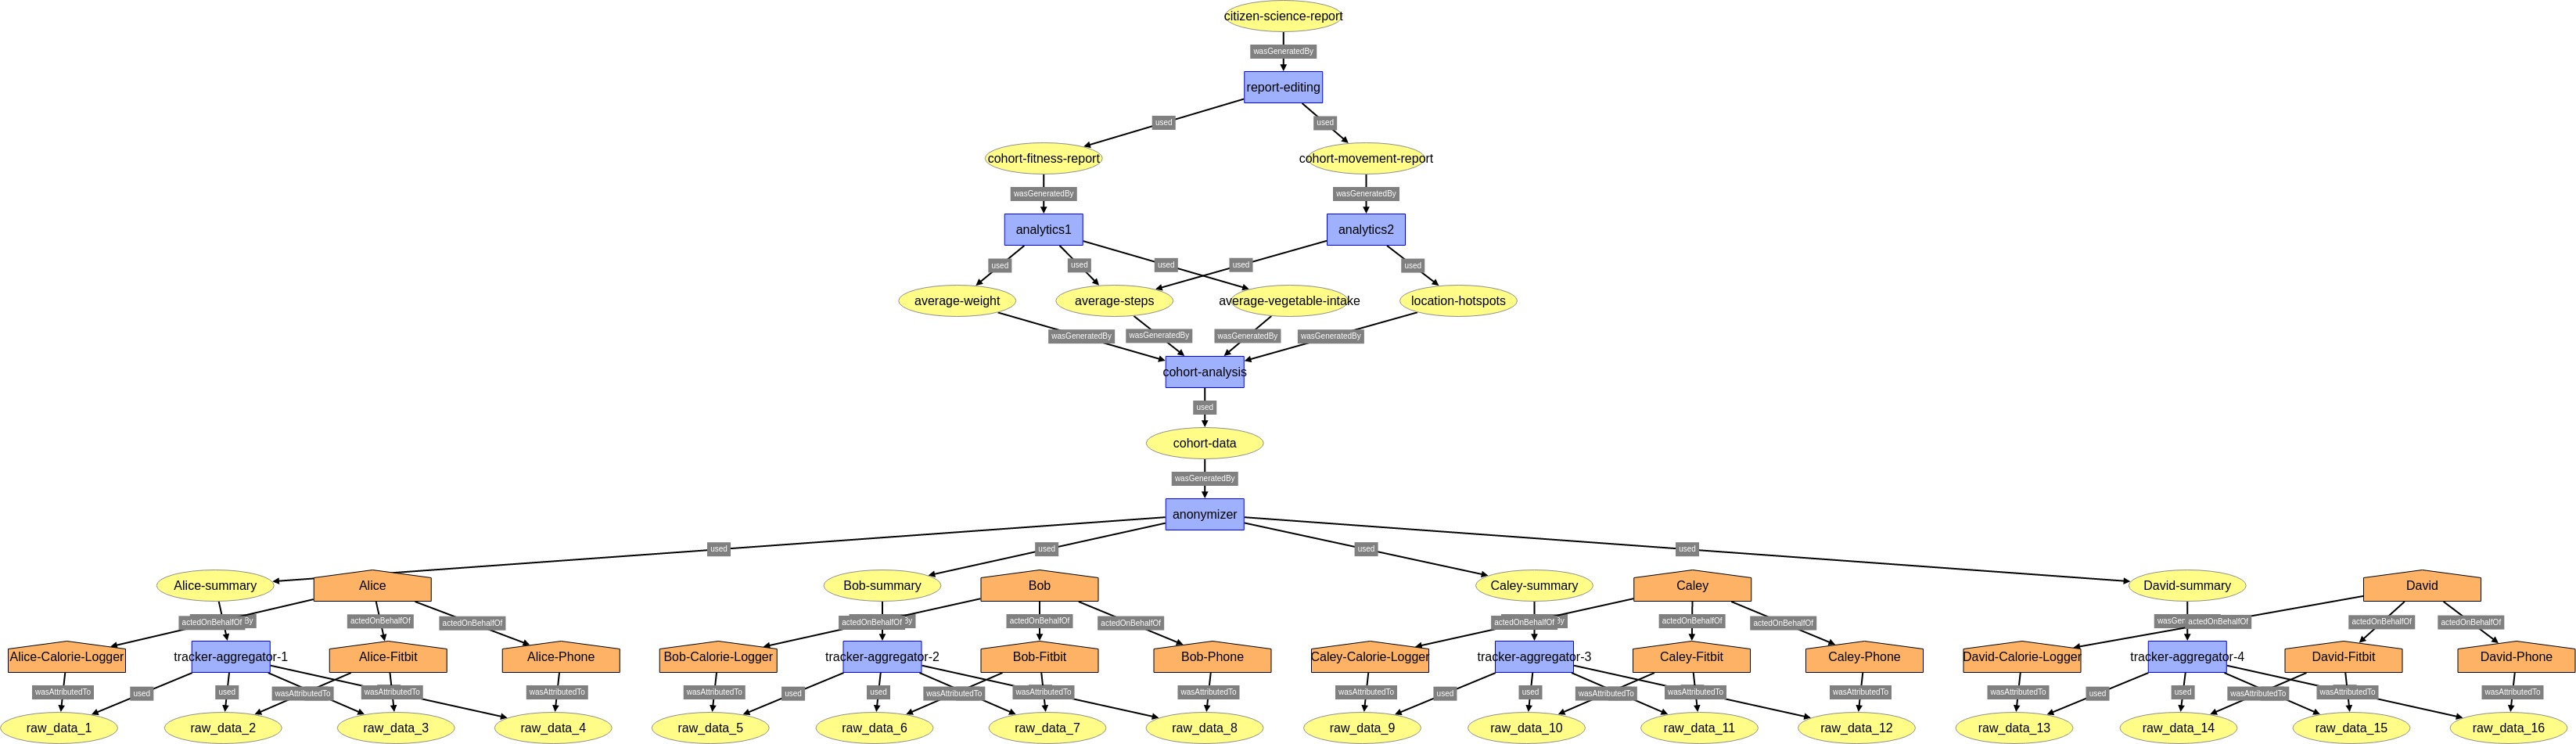
\includegraphics[width=0.8\linewidth]{exercise2}
	\caption{The provenance graph used in scenario 2 showing the lineage of a citizen science report. The top section of the graph is related to the report writing process whilst the fan out  at the bottom shows information stored about five different people.}
	\label{fig:exercise2}
\end{figure}


\subsubsection{Scenario 3: Twitter Data Report}
\label{ssub:Scenario 3: Twitter Data Report}

The third and final exercise expanded on the previous by requiring users to convey information by modifying the graph. This is silghtly different to exercise two which required the participant to \textit{hide} information, instead users had to convey a certain point through a graph. Same as above the first task asked the user to describe the graph, a bit more difficult as the graph was abstract compared to the previous two. The following two tasks where of the following format: \textit{You want to modify the graph in order to convey the following information: <information to convey>}. 

\begin{flushleft}
This provenance graph is an abstract representation of a report based on twitter data. 
\end{flushleft}

\section{Study Results}
\label{sec:study_results}

\begin{table}[h]
	\centering
	\caption{List of question codes and descriptions of each.}
		\def\arraystretch{1.5}
	\label{tab:question-codes}
	\begin{tabu} to \textwidth { | l | X[l] | }
		\hline
		\textbf{Code}& \textbf{Description}  \\	
		\hline
		\hline
		grouping & Activities that involved users grouping or ungrouping nodes (by any means)\\
		\hline
		grouping-group &  When a user grouped a node \\
		grouping-ungroup & When a user ungrouped a node \\
		grouping-complex & When a user grouped a complex set of noes \\
		\hline
		\hline
		graph & Activities related to understanding a graph conceptually \\
		\hline
		graph-explain & Notice and comment on information in the graph. An example is in exercise one where some users noticed that weight data is both manually and automatically logged. This information is not usually relevant to the question. \\
		graph-understanding & Correctly understand a concept from the graph, usually directly in response to a question. \\
		\hline
		\hline
		lineage & Correctly identifying information related to the lienage of a node. \\
		\hline
		lineage-identify & Correctly identified simple lineage. \\
		lineage-implied & Correctly identified lineage passing through multiple entities. \\
		lineage-complex & Correctly identified lineage that was complex, usually identifying multiple nodes. \\
		\hline
		\hline
		interface & When a user uses a specific bit of the ProvOwl interface. \\
		\hline
		interface-export-image & Using the export -> image menu item to save an image of a graph.\\
		interface-os-screenshot & Using the operating system screenshot functionality to save an image of a graph. \\
		interface-rename & Using the rename function (found in the contexual links in a nodes details) to rename a node. \\
		interface-manual-group & Manually group nodes by ctrl+clicking multiple nodes and selecting \textit{group nodes} from the contexual menu. \\
		interface-search-group & Grouping nodes by searching for the nodes they want to use using the search function and then grouping them. \\
		\hline
		\hline
		privacy & Whether a user was privacy concious at all in relation to personal data. \\
		\hline
 
	\end{tabu}
\end{table}
 % plan of question coding etc.

\section{Results} % results

\chapter{Conclusions and Discussion} % discussion and future work
\section{Future Work}
The prototype source code is available on GitHub\footnote{\url{https://github.com/karsai5/ProvOwl}}. The interface is also available online where you can test it with a sample graph\footnote{\url{http://provowl.com/?file=/prov-examples/provn/threenode.provn}}.
We describe features under development to improve usability.

We propose to create a regular expression language to select nodes, as mentioned in the section on challenges. 
This will enable users to select nodes in cases such as:
(i) Select all nodes with the name ``*Feed''
(ii) Select all nodes \textit{not} influencing the ``Summarize'' node
(iii) Select all children of ``Fitness-Summary''.
For large graphs, this could allow for faster user-directed simplification of a graph. 

As an extension of this, the language should describe parametered clustering, so users ask for multiple similar clusters to be formed. For example ``Create clusters from nodes the same depth from the root'' or even using data inside the nodes ``Create clusters from nodes that have the same creation date''.  

This could also impact the way nodes are automatically named. If the user created clusters from nodes that all have the same creation date, the system may infer that the name for the new node should include the creation date.

We also wish to extend the PROV standard to include descriptions of cluster nodes. This would allow a user to cluster nodes manually, export the PROV file with cluster descriptions and then share with someone else. This \textit{extraction}, being able to export your current state of exploration, would allow further exploration from the current state later on or even sharing with other users for further analysis.

\subsection{False Dependencies}
\label{sec:section_name}

In essense clustering is a simple type of graph rewriting that creates an abstraction of a graph and in turn simplifies deatails. This can cause some anomolies such as false dependencies, circular dependencies and mislabelled relationships. 

A false dependency is when a clustering in the graph has caused a newly implied line of linage that falsly suggests that one enetity had influence upon another. This is in violations of the main assumption that provenance records the factual history of data derivation. The opposite of this, removing a dependency, is not such an issue because it is understood that the ability to observe data trasnformations is limited so therefore all provenaance graphs are expected to be partially incomplete. In Figure~\ref{fig:falsedependencies} you can see a simple example that shows a false dependency caused by joinging nodes \texttt{B1} and \texttt{B2} together. It creates a new line of lineage that falsly implies \texttt{A1} and \texttt{A2} where influenced by \texttt{C1} and \texttt{C2}. Technical consequences of false dependencies also include unnecessary checks and recomputation when revisiting dependent entities to reflect corrected or changed source data. For example if the data in \texttt{C1} was found to be incorrect it would be necessary to follow the lineage up to find what entities need to be recomputed, in the case of Figure~\ref{fig:} (B) this would include both \texttt{A1} and \texttt{A2}.

\begin{figure}[H]
	% TODO fix graph
  \begin{subfigure}[t]{0.5\textwidth}
    \centering
    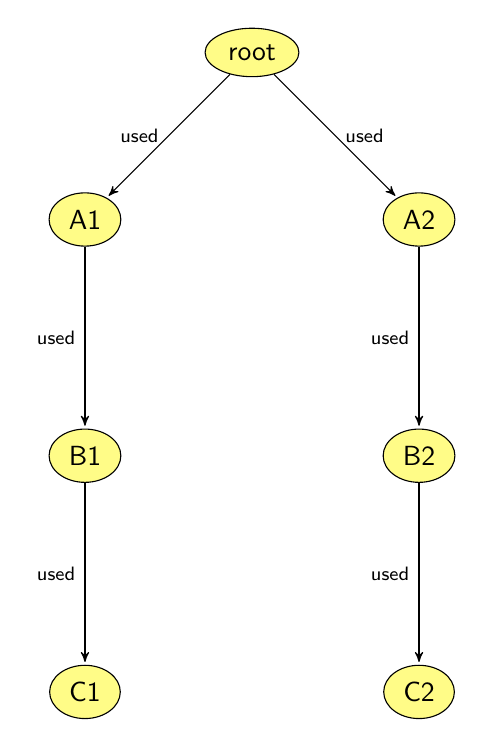
\begin{tikzpicture}
      \node[main node] (root) {root};
	  \node[main node] (A1) [below left of=root] {A1};
      \node[main node] (A2) [below right of=root] {A2};
      \node[main node] (B1) [below of=A1] {B1};
      \node[main node] (B2) [below of=A2] {B2};
      \node[main node] (C1) [below of=B1] {C1};
      \node[main node] (C2) [below of=B2] {C2};
      \path (A1) edge node[left] {used} (B1);
      \path (A2) edge node[left] {used} (B2);
      \path (B1) edge node[left] {used} (C1);
      \path (B2) edge node[left] {used} (C2);
      \path (root) edge node[left] {used} (A1);
      \path (root) edge node[right] {used} (A2);
    \end{tikzpicture}
    \caption{A small example provenance graph that shows two main lines of lineage from the root.}
  \end{subfigure}
  ~
  \begin{subfigure}[t]{0.5\textwidth}
    \centering
    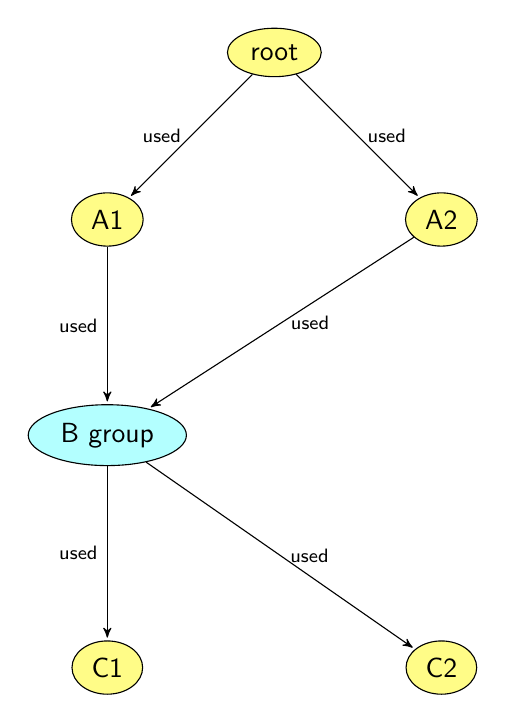
\begin{tikzpicture}
      \node[main node] (root) {root};
      \node[main node] (A1) [below left of=root] {A1};
      \node[main node] (A2) [below right of=root] {A2};
	  \node[main node, group] (CB) [below = 2cm of A1] {B group};
      \node[main node] (C1) [below = 5cm of A1] {C1};
      \node[main node] (C2) [below = 5cm of A2] {C2};
      \path (CB) edge node[left] {used} (C1);
      \path (CB) edge node[right] {used} (C2);
      \path (A1) edge node[left] {used} (CB);
      \path (A2) edge node[right] {used} (CB);
      \path (root) edge node[left] {used} (A1);
      \path (root) edge node[right] {used} (A2);
    \end{tikzpicture}
	\caption{Nodes \texttt{B1} and \texttt{B2} are clustered into the \texttt{B group} composite node.}
  \end{subfigure}
	\label{fig:falsedependencies}
	\caption{When \texttt{B1} and \texttt{B2} are clustered together it creates a false line of lineage that suggests that \texttt{A2} was influenced by \texttt{C2}, this is known as a false dependency.}
\end{figure}

Circular dependencies are another animality that may also occur. This means that the graph is no longer a directed acyclic graph and can cause issues with algorithms that assume the graph is acyclic. It is also in direct violation of the constraints defined in the PROV-CONSTRAINTS W3C document~\cite{}. Figure~\ref{} shows an example of a circular dependency between \texttt{Fitness-Summary group} and \texttt{Summarize}.

The last anomaly that we noticed was that of mislabelled relationships. The labels used to label relationships are specific to the types of nodes the edge is connecting. For example an Entity \textit{was generated by} and Activity, or an Activity was \textit{used} by an Entity. Clustering creates a fourth node type in conjunction with the existing three (Activity, Entity and Agent) and doesn't have any limitation to the labls that can be used on relationships associated with it. This can be confusing to users and can also reveal information about nodes inside a cluster (a used relationship to a cluster node says that there's an entity inside of it). There's also the case of when clustered nodes created multiple relationhips to nodes in common, which relationship label should be picked to represent the relationship? At the moment ProvOwl arbitarily selects one. 

A theoretical formulation of provenance abstraction by clustering has been proposed in~\cite{Missier2014} to discuss this and other problems that occur in clustering, along with simple algorightms for grouping arbitary sets of nodes. In essense the work showed that to avoid false dependencies one must compute a \textit{closure} operation that extends the user-selected nodes with all other nodes that sit on any path amongst these inisial clustering nodes. Combining this work with our user-oriented provenance navigation system can lead to a working correct clustering mechanism. Expanding on the work of this interface to help the user cluster without creating graph anomolies is a challenge we hope to tackle in the future.

\subsection{More powerful regex search}
\label{sec:more_powerful_regex_search}

The challenge is how to create a method for allowing users to cluster a large number of nodes without losing the fine grained control of the above process. We decided to implement a naive search function that runs a regex query on all the properties of a node and hilights any nodes with matching properties.

Future challenges involve allowing users to search for all nodes that match one regex but not another. It would also be useful to only match searches on particular properties of a node, for example a user may only want to match their search on \textit{author} of a node (assuming that property exists\footnote{Breifly discussed in the introduction, the PROV standard allows an arbitraty number of key value properties to be attributed to a node.}). Many users during usability studying requested the ability to cluster all the children of a node, extending from this it would also be useful to allows uers to cluster based on a nodes relationships with other nodes, for example ``Cluster all nodes that match the following regex \texttt{X-tweets|query-X-Time} and are not derived from \texttt{TwitterFeed-time-3}.

Possiblty the biggest challenge in this section would be that of paramaterised clustering. Where a single action by the user would create mutliple clusters. A common clustering we found while studying participants was selecting the entity and the actitvity and creating a composite node of them. In Figure~\ref{fig:search1} they would cluster \texttt{[X-tweets-1, query-X-time-1]}, \texttt{[X-tweets-2, query-X-time-2]} and \texttt{[X-tweets-3, query-X-time-3]} into seperate composite nodes. This would be an ideal use of a paramaterised language that would allow the user to ``group all X-tweets with their corosponding query-X-Time'', however creating a language that is both powerfl and easy to learn and use will be quite a challenge.

A possible future endevour would be automation of clustering. Where the application woudl suggest clusterings based on previous provenance workloads. It may then group together infrequently accessed nodes to make it easier to access infrequently used nodes.

\subsection{Sharing graphs}
\label{sub:sharing_graphs}

In the future I would also like to be able to export the current graph in PROV format with notation for clustered nodes.

\subsection{Server side computation}
\label{sub:server_side_computation}

Server side computation may be a useful feature for the future, a server with higher computational power and resources may be able to find and analyze interesting details about a file. A simple approach to accomplish this would to have the file uploaded to the server, analytics run on the provenance and then results loaded back to the client. For larger provenance files this could be extended to only load sections required for analysis reducing the bandwidth required. The client could render the provenance locally whilst results where computed and then rendered onto the already drawn graph. This would allow the user to begin exploring the graph with minimal delay while extra information is calculated server side.


\printbibliography

\newcommand{\multipdf}[3][]{
	\label{sec:#2}
	\includepdf[pages=1,frame=true,width=\linewidth,pagecommand=\section{#2}]{#3}
	\includepdf[pages=2-#1,frame=true,width=\linewidth]{#3}
}

\newcommand{\singlepdf}[2]{
	\includepdf[pages=1,frame=true,width=\linewidth,pagecommand=\section{#1}]{#2}
}

\begin{appendices}
	\renewcommand{\thesection}{\appendixname~\Alph{section}}

	\singlepdf{Provenance Primer}{pdfs/provenance-primer.pdf}

	\multipdf{Interview Questionnaire}{pdfs/questionnaire.pdf}

	\section{PROV File: IR-Baseline}
	\label{sec:prov_file_ir_baseline}
	
	\lstinputlisting[style=provn]{provn/IR-baseline.provn}

\end{appendices}



\end{document}
